%-----------------------------------------------------------------
%  preamble2016.tex 
%
% UW CENPA Annual Report 
%-----------------------------------------------------------------

%-----------------------------------------------------------------
% Document Structure
%-----------------------------------------------------------------
\documentclass[twoside,11pt]{article}
\textwidth 6.1in 			%fullpage is 6.5
\textheight 8.5in 			%fullpage is 8.9
\addtolength{\topmargin} {-.2in}
\setlength{\oddsidemargin}{0.4in}
\setlength{\evensidemargin}{0cm}
\setlength{\parskip}{.7\baselineskip}
%
% Stop latex from re-creating aux, toc, etc. files
% generally used if you manually created toc or to debug
% \nofiles

%-----------------------------------------------------------------
% Title - header
%-----------------------------------------------------------------
\pagestyle{myheadings}
\markright{\hspace*{\fill} UW CENPA Annual Report 2015-2016  \hspace{\fill} 
DRAFT \hspace{\fill} \today \hspace{\fill}	         % this line for drafts, switch to next line for final
%April 2016 \hspace{\fill}                           % this line for final. set correct year !!!!
}	                                                 % Leave this bracket on a line by itself for convenience.



%-----------------------------------------------------------------
%
%         WATERMARK SECTION - COMMENT OUT FOR FINAL DRAFT
%
% This section puts a watermark on each page. Comment this section for the final draft.
%
%-----------------------------------------------------------------
% Start Draft Watermark and frame
%-----------------------------------------------------------------
\usepackage{draftwatermark}
\SetWatermarkText{CENPA Annual Report DRAFT}
\SetWatermarkScale{2}

%\usepackage{showframe}
%-----------------------------------------------------------------
% End Draft Watermark
%-----------------------------------------------------------------

%-----------------------------------------------------------------
% Packages 
%-----------------------------------------------------------------
% Graphics
% epstopdf is required when using pdfLaTex typesetting.
\usepackage{graphicx,epstopdf}

% Subfigure
% Not needed unless you use a subfigure.  So if you don't have it, comment this line out.
%\usepackage{subfigure}
	
% Simple url inclusion		
\usepackage{url} 
                                
% Mathmode sub and superscript font package
\usepackage{amstext} 


% Amssymb
% this mathmode package was only used for Andreas Knecht's article, AR2011, sec 7.3
%\usepackage{amssymb}	

% Footnoting packages
%
% manyfoot:	provides for multiple footnote declarations
% footmisc:	provides extended fnsymbol footnote list
% perpage:	provides automatic footnote counter resets when needed. 
%	

\usepackage{manyfoot}
\usepackage[stable]{footmisc}
\usepackage{perpage}

% Multi-column packages for the personnel section
%
% multicol: 	provides lists that spans multiple columns
% paralist :	provides /compactitem - removing extra spaces in list output
%
\usepackage{multicol}
\usepackage{paralist}
\usepackage{longtable}

% wrapfig is a text wrapping utility that Duncan used in AR2013, sec 6.5
%
\usepackage{wrapfig}

%-----------------------------------------------------------------
%PATH Stuff
%-----------------------------------------------------------------
\graphicspath{{figures/}{ch1/}{ch2/}{ch3/}{ch4/}{ch5/}{ch6/}{ch7/}{ch8/}{ch9/}{ch10/}{ch11/}}
 \makeatletter
\def\input@path{{.}{ch1/}{ch2/}{ch3/}{ch4/}{ch5/}{ch6/}{ch7/}{ch8/}{ch9/}{ch10/}{ch11/}}
 \makeatother

%-----------------------------------------------------------------
% Footnotes 
%-----------------------------------------------------------------
% Footnotes in author lists, produces symbols
\DeclareNewFootnote{Author}[fnsymbol]  
% Footnotes in text, produces numbers   
\DeclareNewFootnote{Text}[arabic]
% Special footnotes in text to span entire articles (not perpage)             
\DeclareNewFootnote{Misc}[arabic]             

% Makes the author footnotes renumber on a per page basis
\MakePerPage{footnoteAuthor}  
% Makes the text footnotes renumber on a per page basis                  
\MakePerPage{footnoteText}                        

% Make a special CENPA footnote to easily refer to past annual reports by YEAR and PAGE.
\newcommand{\CENPAfoot}[2]{\footnoteText{CENPA Annual Report, University of Washington (#1)  p.~#2.}}

% The following two commands are MACROs to repeat the same footnote within an article.
% They are obsolete with the new footnote system
%\newcommand{\footnoteremember}[2]{\footnote{#2}\newcounter{#1}\setcounter{#1}{\value{footnote}}}
%\newcommand{\footnoterecall}[1]{\footnotemark[\value{#1}]}

%-----------------------------------------------------------------
% Subsection setup 
%-----------------------------------------------------------------

% More stuff for subsubsections
\newlength{\subwidth}					
\setlength{\subwidth}{\textwidth}
\addtolength{\subwidth}{-1.5\parindent}
\newcommand{\subhead}[1]{~\vspace{-\parskip}\par\parbox{\subwidth}{\protect\raggedright{\bf #1}}\vspace{-\parskip} \addcontentsline{toc}{subsubsection}{#1}\par}

%-----------------------------------------------------------------
% Newcommands 
%-----------------------------------------------------------------
% The author block, \auth
%
% The \auth block works as follows. This is a list with one parameter which represents each author entry
% (\item) including whatever footnote(s) might apply. The list has no label (that is the items are not
% enumerated with roman numerals or other symbols), hence the first {} in the declaration. The list is
% automatically left indented in the list environment and the right margin is set even with the document
% margin by default, hence the second {} in the declaration in which the spacing is usually defined. In
% order to keep it from breaking author names the \raggedright qualifier is used within the list environment.
% This structure sets the author block apart from the paragraph structure of the rest of the document. As
% the list encounters entries (\items) defined by the parameter (#1) it enters them into the list until it runs
% out of \item(s). The \par qualifier issues a blank line after the last \item call to end the paragraph in the
% list environment and return to the document environment with \end{list}. At the very end it issues a
% \vspace*{-\parskip} MACRO to place an appropriate space between the \auth block and the first paragraph
% of the article.                     4/1/2011, GTH, GCH
%
\newcommand{\auth}[1]{  \begin{list}{}{}   {\raggedright \item #1 \par}   \end{list}\vspace*{-\parskip}  }
%
% End of the author block

% The following command puts non-bold stuff in table of contents, and makes math bold in heading in text.
% Also avoids nutty hyphen breaks by relaxing right justification. See example article.
\newcommand{\subsecmathbold}[1]{\subsection[#1]{\raggedright \boldmath #1 \unboldmath}}  

% Same but for subsubsections
\newcommand{\subsubsecmathbold}[1]{\subsubsection[#1]{\raggedright \boldmath #1 \unboldmath}}  

% Same as above, but keeps default right justification.
\newcommand{\subsectight}[1]{\subsection[#1]{\boldmath #1 \unboldmath}}  

% The following command formats references to other sections in the document.
%\newcommand{\secref}[1]{(see Sec.~\ref{#1})}
%holman - removed 'see' from secref command 4/2014
\newcommand{\secref}[1]{(Sec.~\ref{#1})}

% The following commands permit a figure or a table to be referenced correctly regardless of nesting level.
% It can float from section to subsection to subsubsection, etc. and it will always be called correctly.
% Each article MUST have a label in the title. The first argument of the figure or table reference is the 
% label in the title of the article and the second argument is the figure or table label.
% The first argument of the figure or table caption is, again, the label in the title and the second argument 
% is the figure or table caption itself

\newcommand{\figref}[2]{Fig.~\ref{#1}-\ref{#2}}   % Note, this prints "Fig."
\newcommand{\figcaption}[2]{\refstepcounter{figure} \hfil \parbox{.9\textwidth}{\small Figure~\ref{#1}-\arabic{figure}. #2 }  \hfil}
\newcommand{\tabref}[2]{Table~\ref{#1}-\ref{#2}}  % Note, this prints "Table."
\newcommand{\tabcaption}[2]{\refstepcounter{table} \hfil \parbox{.9\textwidth}{\small Table~\ref{#1}-\arabic{table}. #2 }  \hfil}

% The following commands, \degrees, \cpp, \MJ, \MJDemo, \snop, \nonubb, \gp, \LS, \RD require a trailing \ in order 
% to insert a space afterward. For example, use \MJ at the end of a sentence and \MJ\ in the middle of a sentence.
%
\newcommand{\degrees}{$^{\circ}$}                                         % makes a correct degree symbol
\newcommand{\cpp}{C\protect\raisebox{.25ex}{++}\ }               % formats C++ correctly
\newcommand{\MJ}{M{\footnotesize AJORANA}}                        % this works for bolding in titles and the toc
\newcommand{\MJDemo}{D{\footnotesize EMON\-STRAT\-OR}} 	% this works for bolding in titles and the toc
\newcommand{\snop}{SNO\protect\raisebox{.25ex}{+}}             % formats SNO+ nicely
\newcommand{\nonubb}  {${0 \nu \beta \beta}$}                       % neutrinoless double beta decay in math mode
\newcommand{\gp}{$g_P^{}$}                                                % MACRO for the muon boys
\newcommand{\LS}{$\Lambda_S^{}$}                                     % MACRO for the muon boys
\newcommand{\RD}{$\Lambda_D^{}$}                                    % MACRO for the muon boys
\newcommand{\iso}[2]{$^{#1}$#2}                                        % Makes a properly formatted isotope symbol e.g. \iso{28}{Si}


% I don't see the following command used anywhere.      4/1/2011, GCH
% \newcommand{\ms}{\ensuremath{\mbox{m}/\mbox{s}^2}} 
 
%-----------------------------------------------------------------
% Counters 
%-----------------------------------------------------------------
% Reset counters for each new article.
\newcommand{\renum}{
\setcounter{figure}{0}
\setcounter{table}{0}
\setcounter{equation}{0}     }
%
% The counters for perpage footnotes are now automatically reset using the perpage package so
% the following command is obsolete.
%\setcounter{footnote}{0}}      
%
%longtable increments the table counter so redefine it to avoid the crash where the table counter increments by 2
%
\let\templongtable\longtable
\renewcommand{\longtable}{\addtocounter{table}{-1} \templongtable}
%
% These next two commands allow deep nesting beyond the \subsubsection level using the \paragraph and 
% \subparagraph levels. It numbers the entries and places them in the table of contents. 1/23/2011, GCH
%
\setcounter{secnumdepth}{5}                     	% this part is the numbering index
\setcounter{tocdepth}{5}                            % this part is the TOC entry
%
% End of the deep nesting command structure                                                

%-----------------------------------------------------------------
% Defines 
%-----------------------------------------------------------------
% A useful Journal MACRO
\def\Journal#1#2#3#4{{#1} {\bf #2}, #3 (#4)}

% Some useful journal names
\def\ADT{At. Data Nucl. Data Tables}
\def\ARN{ Annu. Rev. Nucl. Part. Sci.}
\def\EUP{{ Eur. Phys. J.} A}
\def\NCA{ Nuovo Cimento}
\def\NIM{Nucl. Instrum. Methods }
\def\NIMA{{ Nucl. Instrum. Methods} A }
\def\NPA{{ Nucl. Phys.} A}
\def\NPB{{ Nucl. Phys.} B}
\def\PLB{{ Phys. Lett.}  B}
\def\PRC{{ Phys. Rev.} C }
\def\PPN{ Phys. Part. Nucl.}
\def\PREP{Phys. Rep.}
\def\PRL{Phys. Rev. Lett.}
\def\PRD{{ Phys. Rev.} D }
\def\ZPC{{ Z. Phys.} C }

% End of the annual report preamble2016 MACRO

\begin{document}

% For your article, use section, subsection, etc. counters up to and including the one at the level that your
% article will appear. Ignore the counters nested at the lower levels, they are not needed.
%
\setcounter{section}{2}   % put in your section here.
\setcounter{subsection}{1} % set to your subsection or (subsection-1 if writing at the subsection level).
%\setcounter{subsubsection}{7} % set to your subsubsection or (subsubsection-1 if writing at the subsubsection level).
%\setcounter{paragraph}{7} % set to your paragraph-1 if you are writing at the paragraph level
%
% The example article is for writing at the subsection level to produce paragraph 5.7. 
% The last counter you use should be set to n-1.
%

\subsection {Simulation and analysis activities for the \MJ\ \MJDemo \label{MJDSimArticle}}

\auth{T.\,H.~Burritt,
\underline{M.~Buuck},
C.~Cuesta,
J.\,A.~Detwiler,
J.~Gruszko,
\underline{I.~Guinn},
D.\,A.~Peterson,
R.\,G.\,H.~Robertson,
and T.\,D.~Van Wechel
}

\noindent The UW \MJ\ group under the direction of Dr. Jason Detwiler leads the simulations and analysis effort within the \MJ\ collaboration. Much of the low-level software for data I/O, event building, data processing, and simulation were written by CENPA personnel. Members of our group have played a central role in the building and validation of the background model for the \MJ\ \MJDemo, which informs the radiopurity criteria upon which the experimental design is evaluated. We also participate in the development and implementation of data analysis techniques, geometrical models for Monte Carlo simulations, and data handling, storage, and database technologies. Our efforts over the past year have focused on workflow management, improvements to data processing and cleaning, and the development and use of analysis tools for data from the first commissioning run of the \MJ\ \MJDemo\ Module 1. A significant achievement for the collaboration this past year was the submission for publication of a paper on our muon veto system.

%As the Simulations and Analysis task leader for \MJ, Jason Detwiler oversees the development of the software tools necessary for full data taking. This past year, Detwiler implemented a working group structure to better organize the members of the collaboration around the software tasks at hand. This restructuring has been a great success, and has significantly accelerated the production of the \MJ\ software tools.
\begin{wrapfigure}{r}{0.5\textwidth}
\begin{center}
\hfil  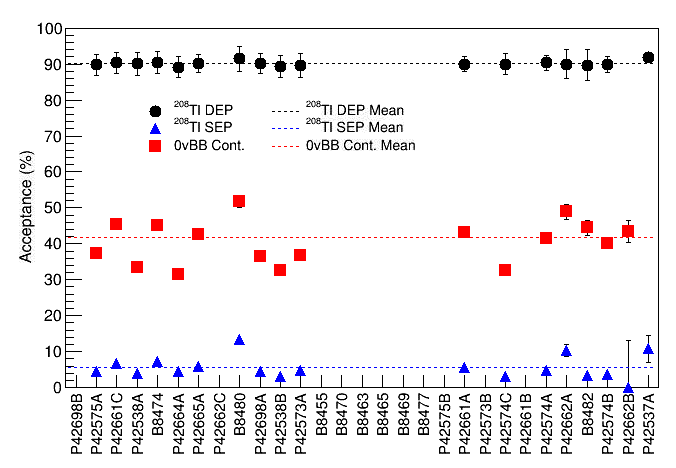
\includegraphics[width=.48\textwidth]{DS1_AoverECut_Efficiency_160330.png} \hfil 
% the following blank line is important

\end{center}
%Sorry Gary, but the default wasn't working with wrapfigure
\refstepcounter{figure} \hfil \parbox{.5\textwidth}{\small Figure~\ref{MJDSimArticle}-\arabic{figure}. A/E acceptances for all detectors in Module 1. The black circles show the acceptance in the \iso{208}{Tl} double-escape peak, which is dominated by single-site interactions. We tune the acceptance there to the expected fraction of \nonubb\ events that are single-site, which is 90\%. The technique is very successful at rejecting events in the \iso{208}{Tl} single-escape peak (blue triangles), which is dominated by multi-site interactions. The effect of the cut on backgrounds in the \iso{76}{Ge} \nonubb-decay region-of-interest is given for each detector by the red squares. }  \hfil

\label{AoE}  %put label{} after \figcaption{}

\end{wrapfigure}

In her role as head of the Data Cleaning and Run Selection working group, Dr. Clara Cuesta has continued to oversee the implementation and evaluation of the Data Cleaning and Run Selection framework for \MJ. Her work in this regard is detailed elsewhere \secref{}.\newline
\indent Dr. Cuesta has also led the development of a pulse-shape based background suppression technique called A/E which analyzes the ratio of the max current in a pulse to the energy collected. Events that produce a single localized energy deposit \--- such as most \nonubb\ decays \--- will have a larger value of A/E than events that deposit energy in multiple locations inside the same detector. We have shown using \iso{228}{Th} calibration data that we are able to reduce our backgrounds using this technique by more than 50\% (see \figref{MJDSimArticle}{AoE}).

Julieta Gruszko has collaborated in the development and largely herself implemented a new technique to tag events that occur near the passivated surface of the \MJ\ detectors. The technique compares the decay of waveforms after the rising edge, looking for differences in the effective decay constant. Preliminary results are presented elsewhere \secref{LAAttE}.
%These events, which could be due to degraded $\alpha$-particles, create some electron-hole pairs in the passivated layer. The holes are collected relatively quickly at the point-contact, but the electrons drift slowly out of the passivated layer, causing a small amount of delayed charge to be collected after the primary rising edge.

\begin{wrapfigure}{l}{0.5\textwidth}
\begin{center}
\hfil  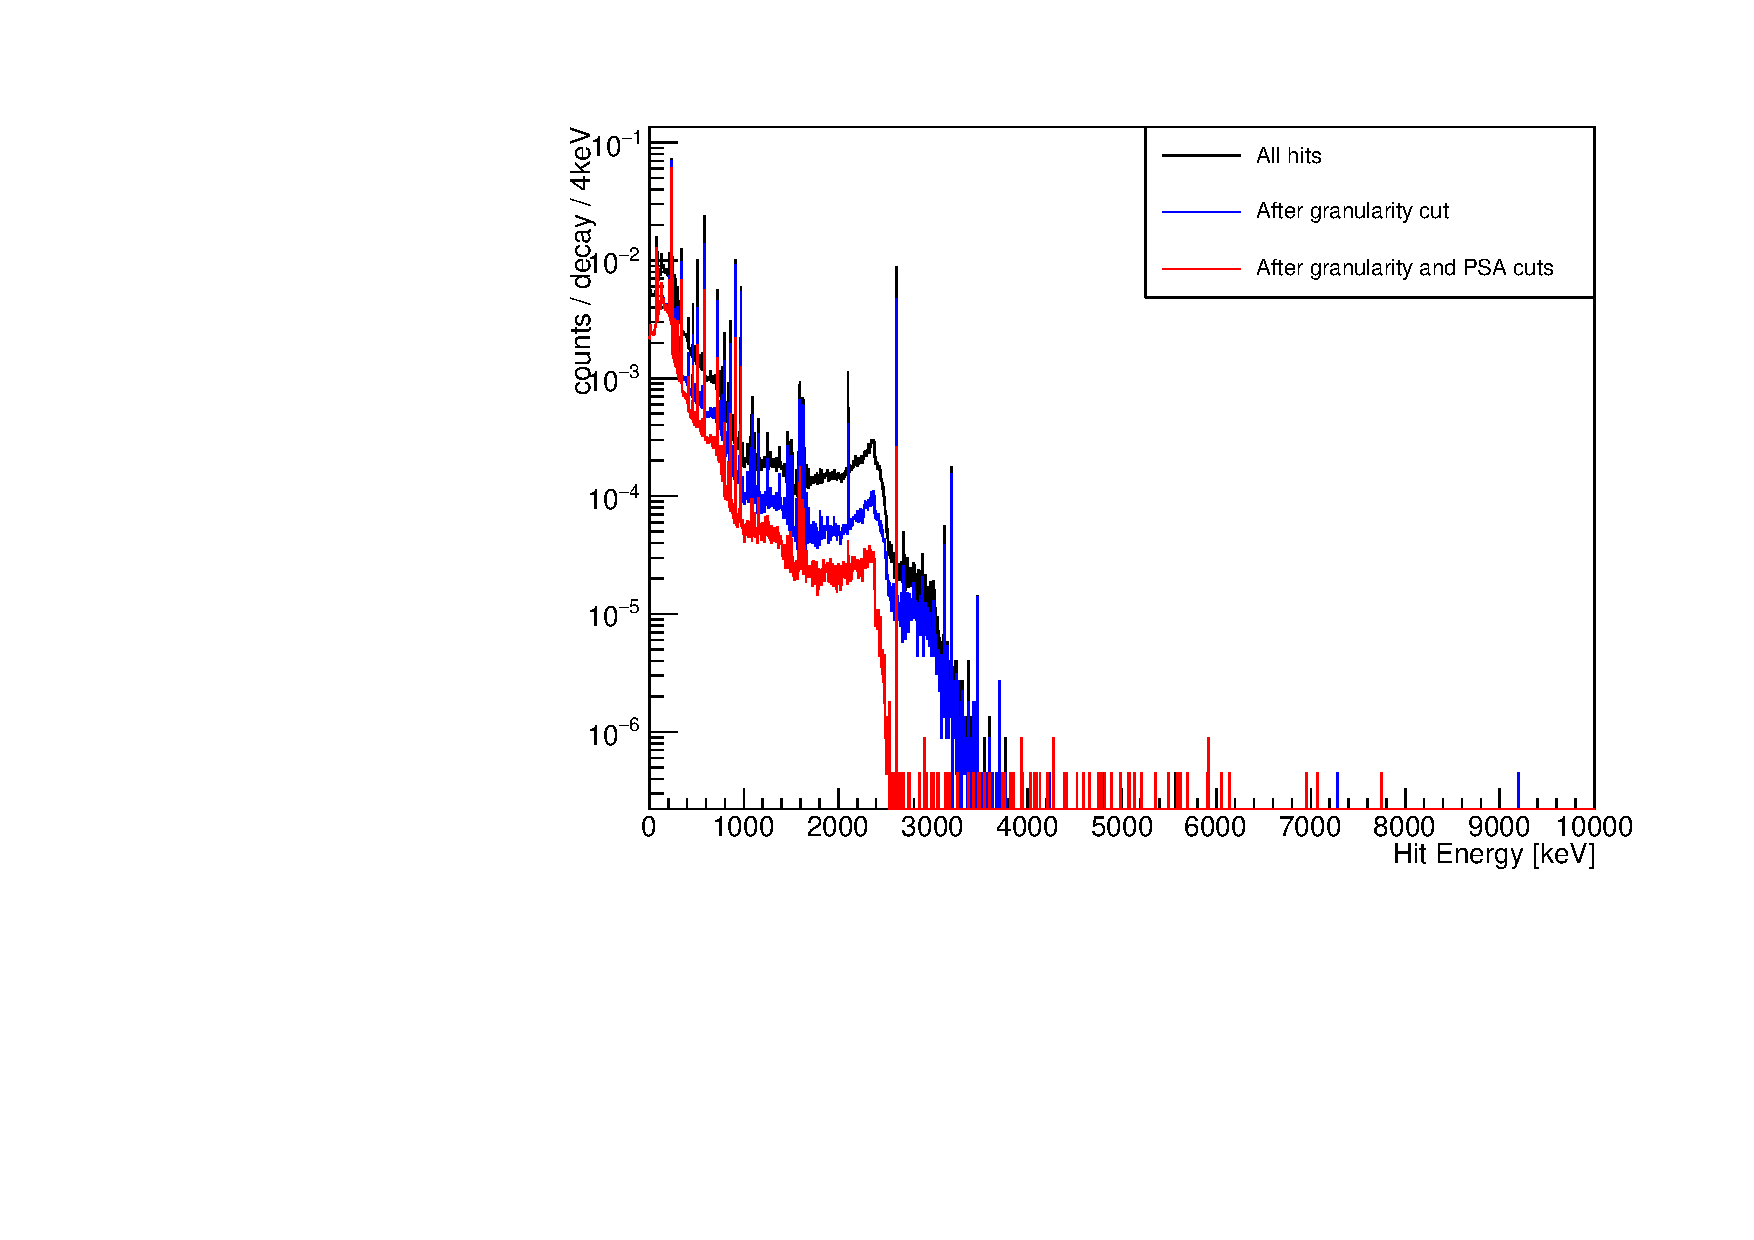
\includegraphics[width=.48\textwidth]{M1DUThCombined.pdf} \hfil 
% the following blank line is important

\end{center}
\refstepcounter{figure} \hfil \parbox{.5\textwidth}{\small Figure~\ref{MJDSimArticle}-\arabic{figure}. A simulation of the efficiency of the Module 1 array of Ge detectors for detecting thorium contamination in the copper detector unit pieces. The black line shows all energy depositions recorded by the array that do not occur in the dead layer of a detector. The blue line has removed events occurring in multiple detectors, and the red line has additionally removed events that are detectable as multi-site within a single detector. }  \hfil

\label{sim}  %put label{} after \figcaption{}

\end{wrapfigure}

Micah Buuck has primarily focused this year on two simulations- and analysis-related activities: a pulse-shape based technique for identifying multi-site backgrounds complementary to A/E, and upgrading the simulations software to produce results on the detector level.\newline
\indent The pulse-shape technique requires the generation of a ``basis library'' of single-site event pulses, which is then used to accept or reject incoming pulses based on a $\chi^2$ fit. He has successfully implemented the software necessary to generate the basis, and has done so on selected sets of calibration data. He is now in the process of quantifying the acceptance of the technique for various kinds of pulse shapes, and tuning input parameters to achieve optimal distinction between single- and multi-site pulses.\newline
\indent Buuck has also modified and upgraded the \MJ\ simulations post-processing software to incorporate detector-specific responses. He updated old code that determines which simulated interactions happen in the detector dead layers, and whether an event is likely to be distinguishable as multi-site. \figref{MJDSimArticle}{sim} is a simulation of the efficiency of the Module 1 array for detecting thorium contamination in the copper detector unit pieces. Each detector has a unique dead layer geometry and drift time mapping (primarily based on the detector shape) whose effects must be applied, before combining the data into a single spectrum. See the figure caption for description of the different lines.
%Micah Buuck has primarily been focused on implementing a pulse-shape-based analysis technique for rejection of background multi-site events. In this capacity, he is a part of the Pulse Shape working group. The technique requires the generation of a ``basis library'' of single-site event pulses, which is then used to accept or reject incoming pulses based on a $\chi^2$ fit. He has successfully implemented the software necessary to generate the basis, and is now working on streamlining the process and applying it to physics data.

Ian Guinn has continued to work on the event builder for the \MJ\ \MJDemo. The event builder has three main responsibilities. First, it converts the raw data files produced by the data acquisition system (ORCA) into ROOT files, known as built files, that are compatible with the \MJ\ software. Second, it combines waveforms and muon veto events that occur at nearby times into a single event, in order to detect coincidences. Finally, it filters out corrupted data that may confuse the main analysis software, a process known as garbage collection. In the last year, Guinn has implemented a builder for the muon veto data. He has also added a checker for built files, which searches for inconsistencies and errors that occur during the building process. Additionally, the event builder is now capable of building multi-sampled waveforms, in which the baseline and falling edge waveforms are sampled at a slower rate than the rising edge. Guinn has also made a number of other improvements and bug-fixes.\newline
\indent Guinn has also implemented a sophisticated algorithm for \MJ\ that fits peaks in the \MJDemo\ energy spectrum. The peak shape is composed of a gaussian, a high-energy exponential tail, a low-energy exponential tail, a flat background, and a step function. The peak fitter is used most importantly in calibrating the energy spectrum of the detectors. Guinn is currently working on extending the peak fitter to fit multiple peaks simultaneously, which will allow for faster and more robust energy calibration. Perhaps insert peakfitter image here?
%Julieta Gruszko has successfully implemented and begun to use new frequency-domain analysis techniques. She will use the techniques to identify and eliminate noise sources and for data cleaning. The resulting noise curves of detector baselines will be used to characterize the detector, to accurately simulate pulses, and for optimum filtering. The tools she developed this year allow researchers to view noise curves over time, which can be used to identify intermittent noise sources and therefore tag events for data cleaning. Average noise curves taken with the Prototype Cryostat system are being used to identify the optimal electronics setup and laboratory conditions for data taking. For an example, see \figref{MJDSimArticle}{Fluorescent_Lights}.
%
%
%\begin{figure}[h]
%\begin{minipage}{.5\textwidth}
%
%\hfil  \includegraphics[width=\textwidth]{MJFluorLights.jpeg} \hfil 
%% the following blank line is important
%
%\figcaption{MJDSimArticle}{A comparison of the white noise levels showed that the use of fluorescent lights in the lab was introducing noise. Following this study, the shielding of module electronics box was improved.}
%
%\label{Fluorescent_Lights}  %put label{} after \figcaption{}
%
%\end{minipage}
%\begin{minipage}{.5\textwidth}
%
%\hfil \includegraphics[width=\textwidth]{MJBGSpectrum.pdf} \hfil
%
%\figcaption{MJDSimArticle}{Full-spectrum background model for the MAJORANA DEMONSTRATOR, with and without analysis cuts.}
%
%\label{MJBGSpectrum}
%
%\end{minipage}
%\end{figure}
%

We are now analyzing the first data to come from the first module of enriched Ge detectors, and have recently commenced blind data taking. Other major activities include software quality assurance tests, utilization of run and detector information stored in our databases, automatic data workflow management, refinement of event building routines, optimization of energy estimation and pulse-shape parameter extraction algorithms, and data monitoring and cleaning routines.
%New assay results have improved the predicted background rate in the 4-keV region of interest surrounding the 2039 keV Q-value for double-beta decay of ${}^{76}$Ge to 3.1 counts/ton-year. Major simulation campaigns are underway to provide up-to-date predictions for the full spectrum we expect to see with enriched detector data. \figref{MJDSimArticle}{MJBGSpectrum} shows the full simulated spectrum, including the effect of analysis cuts. Other major activities include software quality assurance tests, database implementation of run information recording and automatic data workflow management, refinement of event building routines, optimization of energy estimation and pulse-shape parameter extraction algorithms, and data monitoring and cleaning routines.

%% This is a sample for the annual report.  The following things are 
% not standard tex, because of numbering conventions, layout, etc.
%
% PLEASE READ THE FOLLOWING, SPECIFICALLY THE PART ABOUT SPECIAL COMMANDS FOR REFERENCING TABLES AND FIGURES
%
% Do not typeset this LaTex file directly, instead use MakeArticle.tex.
% To typeset, the following files must be in located the same folder:  
%
% preamble2016.tex
% examplefig.eps
% ExampleArticle.tex
% MakeArticle.tex
%
% preamble2016.tex adds the \begin{document} command and defines CENPA specific formatting.
% It also defines the MACRO \auth{} which will format the authors.
%
% 1) Titles must be built as in the example.  Use \section{}, \subsection{}, \subsubsection{},  or \paragraph{}.
%
% 2) Authors go below title, use the \auth{} MACRO as shown in the example. Author footnotes should be done as 
% in the example with Van~Schagen.  The command \, makes a nice space between initials.
%
% 3) Footnotes in the text should be done with the \footnoteText{} command.
% The format for references to journals is shown. Also shown is the reference
% to old annual reports using \CENPAfoot{year}{page}
%
% 4) Figures should be done with the graphicx package (note X not S at the end)
% Use .eps, .pdf, .png, or .jpg files, please
% If you need to put two figures side by side and don't know how, see me.
%
% 5) If you want a table with no reference or caption, just put it in.
%
% 6) Every article must have a label.  Put a \label{} within the title (\subsection{}) as shown below. To reference 
% another article in this report use the \secref{} MACRO to refer to it from the other article. \secref{} will return
% (see Sec. W.X) or (see Sec. W.X.Y) or (see Sec. W.X.Y.Z) depending on the nesting. The parentheses WILL be there.
%
% Figures and tables also use your article label for the numbering scheme.
%
% Use the MACRO \figcaption{articlelabel}{figurecaption} to make the figure caption at any section level.  
% The argument is the text of the figure caption.
% Use the MACRO \figref{articlelabel}{figurelabel} to reference figures at the any section level. The argument is the figure label.
%
% Use the MACRO \tabcaption{articlelabel}{tablecaption} to make the table caption at the subsection level. 
% The argument is the text of the table caption.
% Use the MACRO \tabref{articlelabel}{tablelabel} to reference the tables at any section level. The argument is the table label.
%
% Label your figure or table with something likely to be unique to the annual report.  
% Everybody will have a "figure1" so use something descriptive.  E.g. He6YieldVsBeamCurrent.
%
% The MACRO \degrees makes a degree symbol that looks right
% The MACRO \cpp produces a C++ that looks right
% \iso{13}{N} makes an isotope
% \MJ\ makes small cap Majorana with a trailing space. 
% \MJ makes small cap Majorana without a space. 
% \snop makes a nice representation of SNO+
% \MJDemo Makes the small cap version of Demonstrator
% \nonubb makes neutrinoless double beta decay in math mode
% \gp makes mathmode g sub cap P
% \LS makes mathmode cap Lambda sub cap S
% \RD makes mathmode cap Lambda sub cap D
%
%
%
\subsection{The \iso{4}{He}(\boldmath $\alpha , \gamma $\unboldmath)\iso{8}{Be} experiment \label{articlelabel} }
%
% Please make multi-word titles with the first capitalized only: e.g. \subsection{A title with multiple words about Coulomb's law}
% You naturally capitalize things which would be capitalized in a normal sentence. Note that there is a label for this title. Also note
% the examples of the use of the \iso{}{} MACRO and that it uses the \boldmath MACRO for producing normal text in the TOC and
% bold mathmode in the title.
%
% In this example, \subsection is used as the starting level. Other valid hierarchal constructs are \section, \subsubsection and \paragraph.
% Unless otherwise instructed,  it is safe to leave the document level at \subsection{} when you submit your titles and articles.  
%
\auth{
R.~Hazama, 
K.\,A.~Snover, 
\underline{D.\,W.~Storm},
J.\,P.\,S.~Van~Schagen\footnoteAuthor[1]{Presently at WRQ, Seattle, 98109.}, 
D.\,D.~Victory\footnotemarkAuthor[1], 
and
Z.\,Z.~Zootsuit\footnoteAuthor[2]{Cracker Institute, Crackerville, USA.}
}
% Notice the repeated footnote format for \footnoteAuthor[1]{argument} and footnotemarkAuthor[1]. This author list is
% alphabetized by last name, fully initialed, correctly formatted, and very easy to read.

% Do not indent the first paragraph of each article

\noindent     % This prevents the indentation of the first paragraph. Don't skip the next line.
We are in the process of completing the analysis of the 
high-precision measurement\CENPAfoot{1999}{5} (that's a CENPA annual report footnote, by the way)
of the \iso{4}{He}($\alpha , \gamma$)\iso{8}{Be}
reaction.   We are using the results of Marrs {\it et al}\,\footnoteText{\label{marrs}R.\,E.~Marrs, E.\,G.~Adelberger, and K.\,A.~Snover, Phys. Rev.  C {\bf 16}, 61 (1977).}. %I'm really smart. I just footnoted italicized text so I needed to add a clever little space using \,. Can you see that trick?
I can repeat that last footnote because it's labeled. Isn't that handy? See how this paragraph is not indented? Then you write more text and so on. Try to make it interesting and spell stuff right.

As you can see, this paragraph is indented, while the first one wasn't.
I'm going to use that last footnote again\footref{marrs} like that. Is that easy, or what? The footnotes are renumbered on a per page basis. Some interesting results are given in \tabref{articlelabel}{mytable}. Look at the table this produces. See how it is numbered and captioned.

\begin{table}[h]
\begin{center}
\begin{tabular}{lcr}
Day of week &  hours of sun & hours of rain \\
Monday &	1	& 3 \\
Tuesday & 5  & 7 \\
Friday & 9 & 0 \\
\end{tabular}

\tabcaption{articlelabel}{~~~Local weather conditions for the week of February 35.}
\label{mytable}  %put label{} after \tabcaption{}

\end{center}
\end{table}

And what do you think of \figref{articlelabel}{myFig1}?
Note the figure number and caption are done in an unusual way to enable the numbering to
follow the section numbering.  Be sure that you copy this numbering scheme, substituting only your
own figure and table labels for the last bit.

\begin{figure}[h]

\hfil  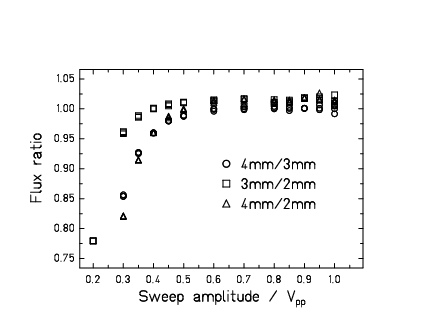
\includegraphics[width=.45\textwidth]{examplefig} \hfil 
% the following blank line is important

\figcaption{articlelabel}{Ratio of beam fluxes through different size apertures, measured with a deuteron beam ($E_d$ = 770 keV).}

\label{myFig1}  %put label{} after \figcaption{}

\end{figure}

Now, for some silly reason, I'm going to reproduce the first table in \tabref{articlelabel}{mytable2} where it is repeated exactly. That's a dumb idea. Why repeat the same table twice? Don't do it in your article, you'll come across as a bonehead. Instead, write smart and clever stuff that will captivate people. This is just an example.

\begin{table}[h]
\begin{center}
\begin{tabular}{lcr}
Day of week &  hours of sun & hours of rain \\
Monday &	1	& 3 \\
Tuesday & 5  & 7 \\
Friday & 9 & 0 \\
\end{tabular}

\tabcaption{articlelabel}{The same local weather conditions again for the week of February 35.}
\label{mytable2} %put label{} after \tabcaption{}

\end{center}
\end{table}



Nobody wrote any \cpp code.  See how weird C++ is typeset? There are MACROs for oddball stuff like \MJ\ and for \snop\ as well. There is one to make \MJ\ end with a period like \MJ. Do you want to typeset 20 degrees~C? Here's how: 20\degrees~C.

Lets write another paragraph to fill up some space.  Back in the old days we did this Annual Report with a typewriter.  {\tt Typewriters look like this. } Need an old annual report footnote?  Here is how\CENPAfoot{1923}{6}. See how the footnotes renumbered to 1 on this new page?




\end{document}
